\documentclass{article}
\usepackage[utf8]{inputenc}
\usepackage{geometry}
\geometry{left=2.0cm,right=2.0cm,top=2.5cm,bottom=2.5cm}
\usepackage{amsmath, amsthm, amssymb, bm, bbm}
\usepackage{mathrsfs}
\usepackage{extarrows}
\usepackage{pifont}
\usepackage{diagbox}
\usepackage{xcolor}
\usepackage{multirow}
\usepackage{graphicx}
\usepackage{hyperref}
\usepackage{float}
\hypersetup{colorlinks=true, linkcolor=blue, citecolor=blue, urlcolor=black}
\usepackage{caption}
\usepackage{braket}
\usepackage{pgfplots}
\usepackage{multirow}
\usepackage{authblk} 
\usepackage{tikz}
\usepackage{cite}
\usepackage{qcircuit}

\newcommand{\abs}[1]{\left| #1 \right|}
\newcommand{\vabs}[1]{\left\| #1 \right\|}
\newcommand{\pbra}[1]{\left( #1 \right)}
\newcommand{\cbra}[1]{\left\{ #1 \right\}}
\newcommand{\sbra}[1]{\left[ #1 \right]}
\newcommand{\abra}[1]{\left\langle #1 \right\rangle}
\newcommand{\supket}[1]{|#1 \rangle\rangle}
\newcommand{\supbra}[1]{\langle\langle #1 |}
\newcommand{\supbraket}[1]{\langle\langle #1 \rangle\rangle}
\newcommand{\tr}[1]{\text{Tr}\left( #1 \right)}
\newcommand{\var}[1]{\text{Var}\left( #1 \right)}



\newtheorem{theorem}{Theorem}
\newtheorem{lemma}{Lemma}
\newtheorem{proposition}{Proposition}
\newtheorem{problem}{Problem}
\newtheorem{corollary}{Corollary}
\newtheorem{claim}{Claim}
\newtheorem{conjecture}{Conjecture}
\newtheorem{definition}{Definition}
\newtheorem{fact}{Fact}
\newtheorem{construction}{Construction}
\newtheorem*{answer}{Answer}
\newtheorem*{example}{Example}
\newtheorem*{counterexample}{Counterexample}
\newtheorem{assumption}{Assumption}

\newcommand{\Ucal}{\mathcal{U}}
\newcommand{\Zcal}{\mathcal{Z}}
\newcommand{\Ocal}{\mathcal{O}}
\newcommand{\Mcal}{\mathcal{M}}
\newcommand{\Pcal}{\mathcal{P}}
\newcommand{\Rcal}{\mathcal{R}}


\newcommand{\Ebb}{\mathbb{E}}
\newcommand{\Rbb}{\mathbb{R}}
\newcommand{\Ibb}{\mathbb{I}}
\newcommand{\Ubb}{\mathbb{U}}
\newcommand{\Cl}{\text{Cl}}
\newcommand{\ii}{\mathrm{i}}
\newcommand{\id}{\mathbbm{1}}



\usepackage{cite}

\title{Shallow fermionic shadow with error mitigation}

\begin{document}

\maketitle

\section{Open question}

\begin{itemize}
    \item [(1)] Can we directly measure $\gamma_S$ with a fermionic quantum device?
\end{itemize}

\section{PPT for CS}

$\Mcal = \Ebb_{\Ucal} \sbra{\Ucal^{-1} M_x \Ucal}  = \Pi_0 + f\Pi_1$
where $f = \frac{\tr{M_x \Pi_1}}{\tr{\Pi_1}} =\frac{1}{2^n+1}$.
\\
\\
$\Mcal^{-1} = \Pi_0 + (2^n+1)\Pi_1$
\\
\\
$\widetilde\Mcal = \Ebb_{\Ucal} \sbra{\Ucal^{-1} M_x \Lambda \Ucal}  = \Pi_0 + f\Pi_1$
where $f = \frac{\tr{M_x \Lambda\Pi_1}}{\tr{\Pi_1}}$
\\
\\
$\Mcal^{-1} = \Pi_0 + f^{-1}\Pi_1$
\\
\\
\begin{align*}
\Ebb_{U\sim \mu_H(4)} U^{\otimes 2} \otimes \bar{U}^{\otimes 2} = \sum_{\sigma,\tau} Wg(\sigma^{-1}\tau)\ket{\sigma}\bra{\tau}
\end{align*}

\section{Preliminaries}
Let $\widetilde{\Mcal}_d$ denote the noisy shallow classical shadow channel with depth $d$ and noise $\Lambda$ for each layer. Let $O_d\in\Rbb^{n\times n}$ represent the orthogonal matrix.

\section{Main results}

\begin{lemma}[Ref. \cite{bertoni2022shallow}]
For $\mu \in \cbra{0,1}^{2n}$, let $\alpha_{\mu,d}\in [0,1]$ be defined as
\begin{equation}
\alpha_{\mu,d} := \Pr_{\Ucal\sim \Ubb_d}\sbra{\Ucal\pbra{P^{(\mu)}}\in \pm \Zcal}=\braket{0|\Ucal(P^{(\mu)})|0}^2,
\end{equation}
then $\widetilde{\Mcal}_d\pbra{P^{(\mu)}} = \frac{(2^n-1)(1-p)^k+1}{2^n}\alpha_{\mu,d}P^{(\mu)}$.
\end{lemma}



\begin{theorem}
In the assumption that the noise for each layer forms a 2-design, the classical shadow for the qubit system can be denoted as
\begin{align}
\widetilde{\Mcal} = 
\end{align}
\end{theorem}


\section{Shallow fermionic classical shadow}

Let
\begin{equation}
\Mcal_d := \int_{Q\in O_d} d\mu(Q) \Ucal_Q^{\dagger} M_z \Ucal_Q. 
\end{equation}
denote the fermionic shadow with depth $d$.

\begin{lemma}
The shallow fermionic shadow has the property
\begin{equation}
\Mcal_d(\gamma_S) = \alpha_{S,d} \gamma_S,
\end{equation}
where 
$\alpha_{S,d} = \int_{Q\sim O_d} d\mu(Q) \abs{\braket{0|U_Q \gamma_S U_{Q}^\dagger|0}}^2.$
\end{lemma}

\begin{proof}
Since Pauli-$X$ is in the matchgate group, we can simplify the shallow fermionic channel as
\begin{align}
\Mcal_d(\gamma_S) &= \int_{Q\sim O_d} d\mu(Q)\sbra{\sum_{b\in\cbra{0,1}^n}\braket{b|U_Q\gamma_S U_Q^\dagger |b} U_Q^\dagger \ket{b}\bra{b}U_Q}\\
&= 2^n\int_{Q\sim O_d} d\mu(Q)\sbra{\braket{0|U_Q\gamma_S U_Q^\dagger |0} U_Q^\dagger \ket{0}\bra{0}U_Q}.
\end{align}

%By a similar technique as Lemma 12 of Ref. \cite{bertoni2022shallow}, we see that 
If $S'$ is not equal to $ S$, 
then there exists a permutation matrix $Q$ such that
\begin{align}
Q|_{S,S} = \Ibb, \quad Q|_{S',S'} = -\Ibb,
\end{align}
and hence
\begin{align}
\quad [\gamma_{S}, U_{Q}] = 0, \quad \cbra{\gamma_{S'}, U_{Q'}} = 0. 
\end{align}
It implies
\begin{align}
\frac{1}{2^n}\tr{\gamma_{S'} \Mcal_d(\gamma_S)} &= 
\int_{Q\sim O_d} d\mu(Q) \braket{0|U_Q \gamma_S U_{Q}^\dagger|0}\braket{0|U_Q \gamma_{s'} U_{Q}^\dagger|0}\\
&=\int_{Q\sim O_d} d\mu(Q) \braket{0|U_Q U_{Q'}\gamma_S U_{Q'}^\dagger U_{Q}^\dagger|0}\braket{0|U_Q U_{Q'}\gamma_{s'} U_{Q'}^\dagger U_{Q}^\dagger|0}\\
&= -\int_{Q\sim O_d} d\mu(Q) \braket{0|U_Q \gamma_S U_{Q}^\dagger|0}\braket{0|U_Q \gamma_{s'} U_{Q}^\dagger|0}.
\end{align}
Hence $\Mcal_d (\gamma_S) = \alpha_{s,d} \gamma_S$.
\end{proof}

\begin{lemma}[Wan et al. \cite{wan2022matchgate}]
Let $Q$ be a matrix uniformly randomly sampled from orthogonal group $\Ocal(n)$, then
\begin{align}
& \int_{Q\sim M_n} d\mu(Q)\sbra{\Ucal_Q} = \supket{\Ibb}\supbra{\Ibb}\\
& \int_{Q\sim M_n} d\mu(Q)\sbra{\Ucal_Q^{\otimes 2}} = \sum_{k=0}^{2n}\supket{\Rcal_k^{(2)}}\supbra{\Rcal_k^{(2)}}\\
& \int_{Q\sim M_n} d\mu(Q)\sbra{\Ucal_Q^{\otimes 3}} = \sum_{
\substack{
k_1,k_2,k_3\geq 0\\
k_1 + k_2 + k_3\leq 2n
}
}\supket{\Rcal_{k_1,k_2,k_3}^{(3)}}\supbra{\Rcal_{k_1,k_2,k_3}^{(3)}}
\end{align}
where
\begin{align}
    &\supket{\Rcal_k^{(2)}} = { 2n\choose k}^{-1/2} \sum_{S\subseteq [2n],|S|=k}\supket{\gamma_S}\supket{\gamma_S}\\
    &\supket{\Rcal_k^{(3)}} = {2n \choose k_1,k_2,k_3,2n-k_1-k_2-k_3}^{-1/2} \sum_{
    \substack{
 S_1, S_2, S_3\subseteq [2n] disjoint\\
 \abs{S_j}=k_j,1\leq j\leq 3
    }
    } \supket{\gamma_{S_1}\gamma_{S_2}}
    \supket{\gamma_{S_2}\gamma_{S_3}}
    \supket{\gamma_{S_3}\gamma_{S_1}}
\label{eq:third_moment}
\end{align}
\label{lem:threemomentsMatchgate}
\end{lemma}

     
\begin{figure}
    \centering
    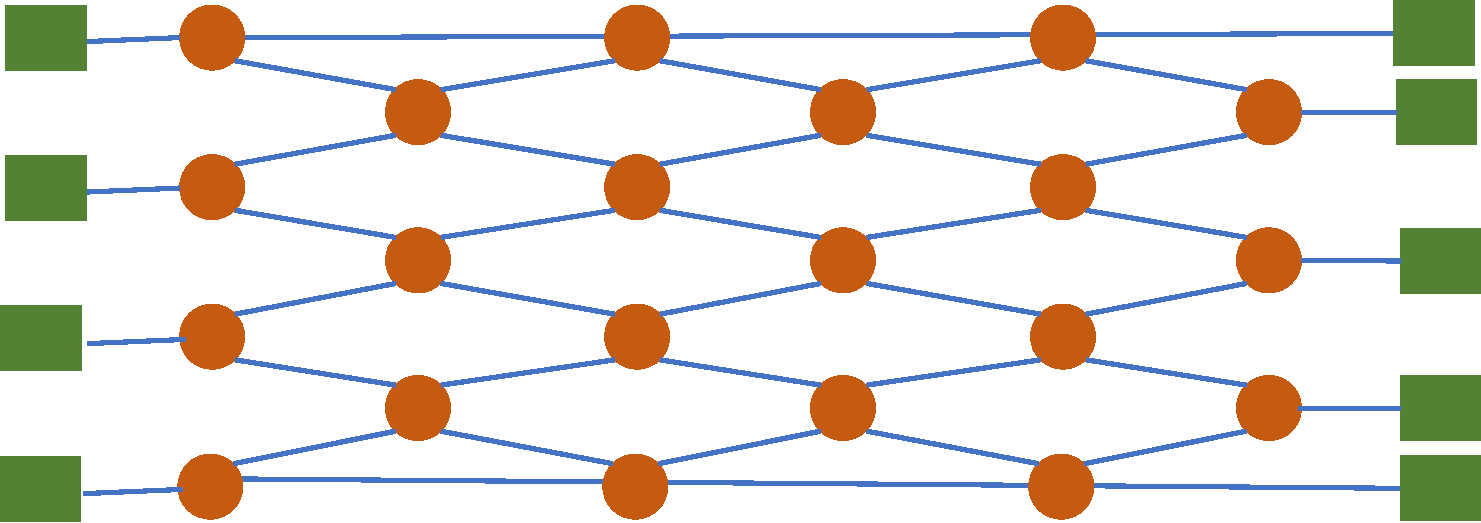
\includegraphics[width = 0.8\textwidth]{shallowCStensor_rep.pdf}
    \caption{Tensor network representation for computing $\alpha_{S,d}$.}
    \label{fig:TNcoefRep}
\end{figure}
% \begin{lemma}
% For the shallow fermionic shadow $\Mcal_d$, the coefficient $\alpha_{S,d}$ can be represented as an MPS with bond dimension at most $n2^{O(d)}$.
% \end{lemma}

% \begin{proof}
% By Lemma \ref{lem:threemomentsMatchgate}, we have 
% \begin{align}
% \int_{Q\sim O_d} \sbra{\Ucal_Q^{\otimes 2}} &= \sum_{k=0}^4\supket{\Rcal_k^{(2)}}\supbra{\Rcal_k^{(2)}}\\
% &= \sum_{k=0}^4\sum_{a_1,a_2}\supket{\Rcal_{k,a_1}^{(2)}} \supket{\Rcal_{k,a_2}^{(2)}} \sum_{a_1,a_2}\supbra{\Rcal_{k,a_1}^{(2)}} \supbra{\Rcal_{k,a_2}^{(2)}} \\
% &:=\sum_{k,a_1,a_2} f(k,a_1,a_2)
% \end{align}
% where the second equation holds since we can decompose $\supket{\Rcal_k^{(2)}}$ as the linear combination of ${4 \choose k}$ terms, and each term is the tensor form for the associated two qubits.
% Then we can represent $\tr{\gamma_S \Mcal_d(\gamma_S)}$ as an MPS with bond dimension at most $n6^{2d}$, as shown in Fig. \ref{fig:TNcoefRep}. 
% \end{proof}

\begin{lemma}
Given any observable $\gamma_S$ and an unknown quantum state $\rho$, let $v$ be the estimation of $\tr{\rho \gamma_S}$ with shallow fermionic shadow $\Mcal_d$.
Then the variance in the average of the input state can be bounded to $1/\alpha_{S,d}.$
\end{lemma}

\begin{proof}

\begin{align}
\var{v} &\leq \Ebb[\abs{v}^2]\\
&= \int_{Q\sim O_d} d\mu Q
 \Ebb_{\rho}\sbra{\sum_b \braket{b|U_Q \rho U_Q^\dagger|b} \abs{\braket{b|U_Q \Mcal_d^{-1} (\gamma_S) U_Q^\dagger|b}}^2}\\
 &=2^{-n}\int_{Q\sim O_d} d\mu Q \sbra{\sum_b \abs{\braket{b|U_Q \Mcal_d^{-1} (\gamma_S) U_Q^\dagger|b}}^2}\\
 &=\frac{1}{\abs{\alpha_{S,d}}^2} \int_{Q\sim O_d}\braket{0|U_Q \gamma_S U_Q^\dagger|0}\braket{0|U_Q \gamma_S^\dagger U_Q^\dagger|0}\\
 &=\frac{1}{\alpha_{S,d}}.
 \end{align}
\end{proof}
\begin{lemma}
$\alpha_{S,d}$ can be bounded to...
\end{lemma}





\begin{itemize}
    \item Bound the complexity to calculate $\alpha_{S,d}$.

We can utilize the MPS method to solve it.

Let matrix $T$ be the probability matrix and the $(j,k)$-th element $T_{j,k}$ denote the probability transforming $P_{j}$ to $P_k$ after performing a unitary $U_Q$ with $Q$ uniformly randomly picked from $P_{2n}$, where $j\in \cbra{0,1}^2$, and $j_l=1$ iff the $l$-th qubit of $\gamma_{S}$ be identity.

    \item Bound the variance.
\end{itemize}

\section{Error mitigation for fermionic shallow CS}

\begin{theorem}
    The noisy classical shadow with any noise model is the same as that with Pauli noise.
\end{theorem}

From Ref. \cite{liu2021benchmarking}, we can get the robust version for shallow classical shadow.




\section{gamma to pauli}
\label{sec: gamma to pauli}

k = 0:

\begin{align*}
	 & \gamma_0 = \Qcircuit @C=1.0em @R=1.0em @!R { \\
	 	 & \qw & \qw\\
	 	 & \qw & \qw\\
\\ }
\end{align*}

k = 1:

\begin{align*}
	 & \gamma_1=\Qcircuit @C=1.0em @R=0.2em @!R { \\
	 	 & \qw & \qw & \qw\\
	 	 & \gate{\mathrm{X}} & \qw & \qw\\
\\ } && \gamma_2=\Qcircuit @C=1.0em @R=0.2em @!R { \\
	 	 & \qw & \qw & \qw\\
	 	 & \gate{\mathrm{Y}} & \qw & \qw\\
\\ }\\ 
	 & \gamma_3=\Qcircuit @C=1.0em @R=0.2em @!R { \\
	 	 & \gate{\mathrm{X}} & \qw & \qw\\
	 	 & \gate{\mathrm{Z}} & \qw & \qw\\
\\ } && \gamma_4=\Qcircuit @C=1.0em @R=0.2em @!R { \\
	 	 & \gate{\mathrm{Y}} & \qw & \qw\\
	 	 & \gate{\mathrm{Z}} & \qw & \qw\\
\\ }
\end{align*}

k = 2:

\begin{align*}
	 & \gamma_1\gamma_2= \ii \Qcircuit @C=1.0em @R=0.2em @!R { \\
	 	 & \qw & \qw & \qw\\
	 	 & \gate{\mathrm{Z}} & \qw & \qw\\
\\ } && \gamma_1\gamma_3=-\ii\Qcircuit @C=1.0em @R=0.2em @!R { \\
	 	 & \gate{\mathrm{X}} & \qw & \qw\\
	 	 & \gate{\mathrm{Y}} & \qw & \qw\\
\\ }\\ 
	 & \gamma_1\gamma_4=-\ii\Qcircuit @C=1.0em @R=0.2em @!R { \\
	 	 & \gate{\mathrm{Y}} & \qw & \qw\\
	 	 & \gate{\mathrm{Y}} & \qw & \qw\\
\\ } && \gamma_2\gamma_3=-\ii\Qcircuit @C=1.0em @R=0.2em @!R { \\
	 	 & \gate{\mathrm{X}} & \qw & \qw\\
	 	 & \gate{\mathrm{X}} & \qw & \qw\\
\\ }\\ 
	 & \gamma_2\gamma_4=\ii\Qcircuit @C=1.0em @R=0.2em @!R { \\
	 	 & \gate{\mathrm{Y}} & \qw & \qw\\
	 	 & \gate{\mathrm{X}} & \qw & \qw\\
\\ } && \gamma_3\gamma_4=\ii\Qcircuit @C=1.0em @R=0.2em @!R { \\
	 	 & \gate{\mathrm{Z}} & \qw & \qw\\
	 	 & \qw & \qw & \qw\\
\\ }
\end{align*}

k = 3:

\begin{align*}
	 & \gamma_1\gamma_2\gamma_3=\ii\Qcircuit @C=1.0em @R=0.2em @!R { \\
	 	 & \gate{\mathrm{X}} & \qw & \qw\\
	 	 & \qw & \qw & \qw\\
\\ } && \gamma_1\gamma_2\gamma_4=\ii\Qcircuit @C=1.0em @R=0.2em @!R { \\
	 	 & \gate{\mathrm{Y}} & \qw & \qw\\
	 	 & \qw & \qw & \qw\\
\\ }\\ 
	 & \gamma_1\gamma_3\gamma_4=\ii\Qcircuit @C=1.0em @R=0.2em @!R { \\
	 	 & \gate{\mathrm{Z}} & \qw & \qw\\
	 	 & \gate{\mathrm{X}} & \qw & \qw\\
\\ } && \gamma_2\gamma_3\gamma_4=\ii\Qcircuit @C=1.0em @R=0.2em @!R { \\
	 	 & \gate{\mathrm{Z}} & \qw & \qw\\
	 	 & \gate{\mathrm{Y}} & \qw & \qw\\
\\ }
\end{align*}

k = 4:

\begin{align*}
	 & \gamma_1\gamma_2\gamma_3\gamma_4=\Qcircuit @C=1.0em @R=0.2em @!R { \\
	 	 & \gate{\mathrm{Z}} & \qw & \qw\\
	 	 & \gate{\mathrm{Z}} & \qw & \qw\\
\\ }
\end{align*}




\section{Representation of 2-fold twirling}
\label{sec: representation of 2fold twirling}

\newcommand{\supketbra}[2]{
    \supket{#1 } \supket{#1 } \supbra{#2} \supbra{#2} 
}
\newcommand{\T}[2]{ T^{#1}_{~~#2}  }
Here, we aim to give a representation of $\int d\mu(Q)\Ucal_Q^{\otimes 2}$. Due to Lemma. \ref{lem:threemomentsMatchgate}, we have
\begin{align*}
    \int_{Q\sim M_n} d\mu(Q)\Ucal_Q^{\otimes 2} =& \supketbra{\gamma_\emptyset}{\gamma_\emptyset}
    + \frac{1}{4} \sum_{i,j} \supketbra{\gamma_i}{\gamma_j}\\
    &+ \frac{1}{6}\sum_{\substack{i_1\neq i_2 \\ j_1\neq j_2}}\supketbra{\gamma_{i_1}\gamma_{i_2}}{\gamma_{j_1}\gamma_{j_2}} \\
    &+ \frac{1}{4}
    \sum_{\substack{i_1\neq i_2, j_1 \neq j_2 \\ 
        i_1\neq i_3, j_1 \neq j_3 \\
        i_2\neq i_3, j_2 \neq j_3} 
    }
    \supketbra{\gamma_{i_1}\gamma_{i_2}\gamma_{i_3}}{\gamma_{j_1}\gamma_{j_2}\gamma_{j_3}}\\
    &+ \supketbra{\gamma_1\gamma_2\gamma_3\gamma_4}{\gamma_1\gamma_2\gamma_3\gamma_4}
\end{align*}

Plugging the table in Sec.~\ref{sec: gamma to pauli}, we present the two-fold twirling to the Pauli basis. Denote the twirling as a $4$-bond tensor as the following rule,
\begin{equation}
    \T{ij}{ab} = \supbra{P^{(a,b)}}\supbra{P^{(a,b)}}\int_{Q\sim M_n} d\mu(Q)\Ucal_Q^{\otimes 2} \supket{P^{(i,j)}}\supket{P^{(i,j)}},
\end{equation}
where $(a,b), (i,j)\in \{(b_1, b_2)\mid b_1, b_2 \in \{0,1\}\}$. We also write $\T{XY}{YZ}$ instead of $\T{(1,1), (0,1)}{(1,0), (1,1)}$ for simplification. 

We write down every element of tensor $T$, which is shown in Table.~\ref{table: tensor T}. 
Here, we give an example of the calculation of $\T{IZ}{XX}$. 
\begin{align*}
    T^{IZ}_{XX} =& \supbra{XX}\supbra{XX} \int_{Q\sim M_n} d\mu(Q)\Ucal_Q^{\otimes 2} \supket{IZ}\supket{IZ}\\
    =& \supbra{\gamma_2\gamma_3}\supbra{\gamma_2\gamma_3} (-\ii)^2 \cdot \int_{Q\sim M_n} d\mu(Q)\Ucal_Q^{\otimes 2} \cdot (-\ii)^2 \supket{\gamma_1\gamma_2}\supket{\gamma_1\gamma_2}\\
    =& \frac{1}{6}\supbra{\gamma_2\gamma_3} \sum_{\substack{i_1\neq i_2 \\ j_1\neq j_2}}\supketbra{\gamma_{i_1}\gamma_{i_2}}{\gamma_{j_1}\gamma_{j_2}} \supket{\gamma_1\gamma_2}\supket{\gamma_1\gamma_2}\\
    = & \frac{1}{6}
\end{align*}
From the first line to the second line, we use the correspondence relation in Sec.~\ref{sec: gamma to pauli}, $\supket{IZ} = -\ii \supket{\gamma_1\gamma_2}$, $\supket{XX} = \ii \supket{\gamma_2\gamma_3}$. Then, terms $\supket{\gamma_{S_1}}\supbra{\gamma_{S_1}}\supbra{\gamma_{S_2}}\supbra{\gamma_{S_2}}$ in $\int d\mu(Q)\Ucal_Q^{\otimes 2}$ cancel if $|S_1|,  |S_2| \neq 2$.   

\begin{table}[]
\begin{tabular}{|c|c|c|c|c|c|c|c|c|c|c|c|c|c|c|c|c|}
	\hline
	T  &II &IX &IY &IZ &XI &XX &XY &XZ &YI &YX &YY &YZ &ZI &ZX &ZY &ZZ \\ \hline
    II & 1 &   &   &   &   &   &   &   &   &   &   &   &   &   &   &   \\ \hline
    IX &   &1/4&1/4&   &   &   &   &1/4&   &   &   &1/4&   &   &   &   \\ \hline
    IY &   &1/4&1/4&   &   &   &   &1/4&   &   &   &1/4&   &   &   &   \\ \hline
    IZ &   &   &   &1/6&   &1/6&1/6&   &   &1/6&1/6&   &1/6&   &   &   \\ \hline
    XI &   &   &   &   &1/4&   &   &   &1/4&   &   &   &   &1/4&1/4&   \\ \hline
    XX &   &   &   &1/6&   &1/6&1/6&   &   &1/6&1/6&   &1/6&   &   &   \\ \hline
    XY &   &   &   &1/6&   &1/6&1/6&   &   &1/6&1/6&   &1/6&   &   &   \\ \hline
    XZ &   &1/4&1/4&   &   &   &   &1/4&   &   &   &1/4&   &   &   &   \\ \hline
    YI &   &   &   &   &1/4&   &   &   &1/4&   &   &   &   &1/4&1/4&   \\ \hline
    YX &   &   &   &1/6&   &1/6&1/6&   &   &1/6&1/6&   &1/6&   &   &   \\ \hline
    YY &   &   &   &1/6&   &1/6&1/6&   &   &1/6&1/6&   &1/6&   &   &   \\ \hline
    YZ &   &1/4&1/4&   &   &   &   &1/4&   &   &   &1/4&   &   &   &   \\ \hline
    ZI &   &   &   &1/6&   &1/6&1/6&   &   &1/6&1/6&   &1/6&   &   &   \\ \hline
    ZX &   &   &   &   &1/4&   &   &   &1/4&   &   &   &   &1/4&1/4&   \\ \hline
    ZY &   &   &   &   &1/4&   &   &   &1/4&   &   &   &   &1/4&1/4&   \\ \hline
    ZZ &   &   &   &   &   &   &   &   &   &   &   &   &   &   &   & 1 \\ \hline
		\end{tabular}
    \caption{Values of tensor $T$. The head of columns represents the input of $T$ while the head of rows represents the output of $T$. For example, the value in row `XY' and column `YZ' represent $\T{(1,1), (0,1)}{(1,0), (1,1)}$.  The blank space represents the value is $0$.    }
\label{table: tensor T}
\end{table}


\section{Calculate $\alpha$}
\begin{lemma}
\label{lemma: gamma dagger}
    \begin{equation} 
        \gamma_S^\dagger = (-1)^{\frac{|S|(|S|-1)}{2}}\gamma_S
    \end{equation}
\end{lemma}
\begin{proof}
    \begin{align*}
        \gamma_S^\dagger =& \Big(
            \gamma_{l_1}\gamma_{l_2}\cdots \gamma_{l_{|S|}}
        \Big)^\dagger\\
        =& \gamma_{l_{|S|}}\gamma_{l_{|S|-1}}\cdots \gamma_{l_1}
    \end{align*}
    Because $\{\gamma_i, \gamma_j\} = 2\delta_{ij}$, it will generate a coefficient $(-1)^{|S|-1}$ when we swap the $\gamma_{l_1}$ to the first place. Thus, we have
    \begin{align*}
        \gamma_S^\dagger=& (-1)^{|S|-1}\gamma_{l_1}\gamma_{l_{|S|}}\gamma_{l_{|S|-1}}\cdots \gamma_{l_2}\\
        =& (-1)^{|S|-1 + |S|-2} \gamma_{l_1}\gamma_{l_2}\gamma_{l_{|S|}}\gamma_{l_{|S|-1}}\cdots \gamma_{l_3}\\
        =& (-1)^{\frac{|S|(|S|-1)}{2}}\gamma_S
    \end{align*}
    
\end{proof}

Base on Lemma \ref{lemma: gamma dagger}, the expression of $\alpha$ becomes
\begin{align*}
    \alpha_{S,d} =& (-1)^{\frac{|S|(|S|-1)}{2}} \int_{Q \sim O_d} d\mu(Q) 
    \bra{0}U_Q \gamma_SU_Q^\dagger\ket{0}^2\\
    =& (-1)^{\frac{|S|(|S|-1)}{2}} 2^n \int_{Q \sim O_d} d\mu(Q) 
    \supbra{0,0} \Ucal_Q\otimes\Ucal_Q \supket{\gamma_S\gamma_S} \\
    =& (-1)^{\frac{|S|(|S|-1)}{2}} 2^n  \supbra{0,0}  \pbra{\int_{Q \sim O_d}d\mu(Q)\Ucal_Q^{\otimes 2}} \supket{\gamma_S\gamma_S}.
\end{align*}
Now, we focus on dealing with $\int d\mu(Q)\Ucal_Q^{\otimes 2}$. In Sec.~\ref{sec: representation of 2fold twirling}, we give a tensor representation of $\int_{M_2} d\mu(Q)\Ucal_Q^{\otimes 2}$. Let the two-fold twirling of a layer of match gates be $T^{(2)}_l$, where
\begin{equation}
    T^{(2)}_l := \begin{cases}
        T^{\otimes \lfloor \frac{n}{2}\rfloor}   ~~& l \mod{2} = 1\\
        \id_2 \otimes T^{\otimes \lfloor \frac{n-1}{2}\rfloor}\otimes \id_0   ~~& l \mod{2}  = 0\\
    \end{cases}.
\end{equation}

Then, we could bound the $\alpha$ to $1/6^d$
\begin{align*}
    \alpha_{S,d} =& \supbra{0,0} \int_{Q\sim Q_d} d\mu(Q)\Ucal_Q^{\otimes 2} \supket{\gamma_S,\gamma_S} = \supbra{0,0} \prod_{1\leq l\leq d} T^{(2)}_l\supket{\gamma_S,\gamma_S} \\
    \geq & \inf\{\supbra{\psi, \psi} T^{(2)}_l \supket{\phi, \phi} \mid ||\supket{\psi}|| = ||\supket{\phi}|| = 1 \}^d \\
    \geq & \frac{1}{6^d}
\end{align*}




\bibliographystyle{unsrt}
\bibliography{ref}

\end{document}
